\clearpage{\pagestyle{empty}\cleardoublepage}		% Begin from odd page
\chapter{Introduction}
\setcounter{page}{1}
\label{intro:chap}

\begin{flushright}
\textit{"Except near the electrodes, where there are sheaths containing very few electrons, the ionized gas contains ions and electrons in about equal numbers so that the resultant space charge is very small. We shall use the name \textbf{plasma} to describe this region containing balanced charges of ions and electrons."}~\cite{langmuir1929tonks}
\end{flushright}
\rightline{-- Irving Langmuir, chemist $\&$ physicist, Nobel Chemistry Prize winner}
\vspace{1cm}
%
%======================================================
\section{General Introduction}
\label{intro:sec:backgroung}
\subsection{Definition of plasma and its properties}
Plasma is the fourth state of material that exists widely in the universe. Typical phenomena of natural plasma are lightning and aurora that humans have already observed. However, these lightning and aurora plasmas only exist in the ionosphere that is far from the earth surface. Except the man-made plasma in the laboratory, natural plasmas are rarely on the earth, while at least $99\%$ of the matter in the universe is in the state of plasma according to Saha equation~\cite{chen1986plasma,saha1920ionisation}(as below in equation \ref{intro:eq:1}), from the plasma in the vicinity of black hole accretion disk, to the relativistic plasma near the Pulsar, from interstellar medium filled sparsely in the intergalactic space, to the solar wind and the Sun that are familiar with humans beings. The Saha equation, named after the Indian astrophysicist Meghnad Saha, estimates the ionization degree of matter in the universe, proving that $99\%$ of the medium in nature exists in the plasma state. The Saha ionization equation is shown as below:
\begin{equation}\label{intro:eq:1}
\frac{n_{i+1}n_e}{n_i} = \frac{2}{\lambda^3}\frac{g_{i+1}}{g_i}e^{-(\epsilon_{i+1}-\epsilon_i)/k_BT}
\end{equation}
where $n_e$ is the electron density, $T$ is the gas temperature, $k_B$ is the Boltzmann constant, $n_i$ is the density of atoms in the i-th state of ionization, $g_i$ is the degeneracy of states for the ions $i$, $\epsilon_i$ is the energy required to remove i electrons from an atom, $\lambda$ is the thermal de Broglie wavelength of electron, defined as $\lambda \equiv\sqrt{h^2/(2\pi m_ek_BT)}$.\\[12pt]
While in our real life, where the rest $1\%$ of the plasma exists, it was already observed by our ancestors that the flame, lightning and aurora belong to some specific kinds of plasmas. And nowadays, with the development of science and technology, more and more man-made plasmas have been created in the laboratory. For example, thanks to the glow discharge plasma, the neon lights appearing in the shopping malls and along the streets add to the brightness of the night in urban cities. Moreover, there are a variety of plasmas, such as the magnetic confinement fusion plasma in Tokamak, the laser inertial confinement plasma, space plasma, dusty plasma, industrial plasma, etc. In addition, plasma ranges over wide parameters both in temperature and density. For example, the density of the weak plasma such as astrophysical plasma is between $10^8$ to $10^{10}$ $\text{cm}^{-3}$, with the temperature at only a few thousand Celsius degrees, while in the center of the Sun, the plasma density can be as high as $9\times10^{25}$ $\text{cm}^{-3}$, and the temperature at 150 million Celsius degrees. A figure of plasmas in a wide range of density and temperature parameters is shown in figure \ref{intro:fig:1}.
\begin{figure}[H]
\centering
   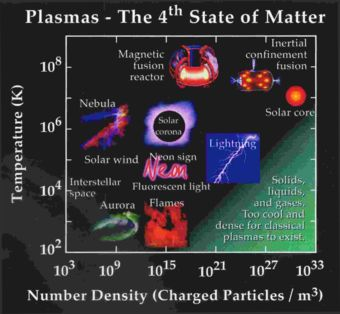
\includegraphics[width=0.5\textwidth]{./03.Introduction/fig/plasma_parameter.jpg}
   \caption{Plasma Parameters}
   \label{intro:fig:1}
\end{figure}
%% (source: \href{https://www.plasmas.org/})
\noindent
The term "plasma" was first introduced by Irving Langmuir and Lewi Tonks in 1928, to describe the gas discharge phenomenon they observed in a gas discharge tube where the ions and electrons are in about equal numbers. The name "plasma" comes from the Greek word $\pi\lambda\alpha\sigma\mu\alpha$, meaning "to mold" or "to shape". Langmuir who was proficient in Greek used the word "plasma" in analogy with the blood because the transport of electrons and ions in a plasma resembles "the way blood plasma carries red and white corpuscles and germs"~\cite{langmuir1929tonks}. Besides, Langmuir also made many contributions to the gas discharge physics, including the Langmuir probe techniques. To some extent, this name reflects the fluid properties of plasma. However, in the early days the physical term "plasma" was often mistakenly associated with the pharmaceutical industry due to the blood meaning in plasma.\\[12pt]
Generally speaking, plasma refers to partially or fully ionized gases. And from a perspective of condensed matter, plasma is thought to be the fourth matter followed by solid, liquid and gas. In a view of electrodynamics, the plasma is an aggregate of large quantities of charged particles. In the plasma, the interaction between particles is mainly the Coulomb force in a long range distance other than nuclei forces inside the atoms, which indicates that the forces between plasma involve long range interactions of many bodies and also couple with the electromagnetic fields. However, this interpretation cannot exactly define what is plasma in the final analysis. Because there is always a certain degree of ionization in the gas. A definition in F.F.Chen's well-known textbook \textit{Introduction to Plasma Physics and Controlled Fusion: Volume 1}: A plasma is a quasi-neutral gas of charged and neutral particles which exhibits collective behavior~\cite{chen1986plasma}. To be noted, plasmas have to satisfy some criteria such as quasi-neutrality, Debye length, plasma oscillation frequency, otherwise, they are simply simple ionized gases. In the next section, the plasma criteria will be introduced.


\subsection{Quasi-neutrality of plasma}
Plasma

\subsection{Debye shielding and Debye length}
In plasmas,

\subsection{Plasma oscillation frequency}
Irving Langmuir 

\subsection{Summary}
To sum up

%======================================================
\section{Research Background}
\subsection{A Brief history of gas discharge}
As mentioned in the previous section
\begin{table}[H]
\centering
\caption{Classification of gas discharges}
\scalebox{0.9}{
\begin{tabular}{lp{3cm}p{3cm}p{3cm}p{3cm}}
\hline Types             & Frequency range     & Gas pressure   &  Typical example\\
\hline Constant electric & low frequency (f$<$1 MHz)    &  0.1-10 torr   &  Glow discharge\\
\hline Radio frequency   & $10^6-10^8$ Hz (usually 13.56 MHz) & 0.1 Pascal to a few atmosphere &  Capacitively coupled plasma discharge\\
\hline Microwave range & $10^9-10^{11}$ Hz (usually 2.45 GHz) &  0.1 Pascal to a few atmosphere  &  Microwave discharge \\
\hline Optical range & from far infrared to ultraviolet light & moderate, high pressure & Laser discharge\\
\hline
\end{tabular}}
\label{intro:tab:1}
\end{table}


\subsection{An Introduction to microwave discharge}
Microwave discharge 


\subsection{Industrial applications of microwave plasma}
With the development 

%======================================================
\section{Research Status}
\subsection{Experimental observations}
In the early studies 

\subsection{Simulation geometry}
The schematic figure

\subsection{Theoretical modeling and numerical methods}
The physical model applied in this thesis is the plasma fluid model~\cite{chen1986plasma,lieberman2005,chen2013}. The general description of plasma models are single particle motion, kinetic theory, and fluid theory. The ideal MHD equations of plasma fluid model can be written as:
\begin{equation}\label{intro:eq:14}
\left\{
        \begin{array}{lr}
         \frac{\partial\rho}{\partial t} + \nabla\cdot(\rho\mathbf{u}) = 0\\
          \rho\frac{d\mathbf{u}}{dt} = -\nabla p + \mathbf{J}\times\mathbf{B}\\
          \frac{d}{dt}(p\rho^{-\gamma}) = 0\\
          %\nabla\times\mathbf{E}= -\frac{\partial\mathbf{B}}{\partial t}\\
          %\nabla\times\mathbf{B} = \mu_0\mathbf{J}\\
          %\mathbf{J} = \sigma(\mathbf{E}+\mathbf{u}\times\mathbf{B})
        \end{array}
\right.
\end{equation}

%======================================================
\section{The Structure of This Thesis}
In this thesis, 

%======================================================
\section{Conclusion}
As an introduction.